%% Преамбула TeX-файла
\bibliographystyle{ugost2008}

% 1. Стиль и язык
\documentclass[utf8x, 14pt]{G7-32} % Стиль (по умолчанию будет 14pt)

\usepackage{indentfirst}
\usepackage{import}
\usepackage{indentfirst}
\usepackage{float}
\usepackage{makecell}
\usepackage{pgfplots}
\usepackage{tikz}

% Остальные стандартные настройки убраны в preamble.inc.tex.
\sloppy

% Настройки стиля ГОСТ 7-32
% Для начала определяем, хотим мы или нет, чтобы рисунки и таблицы нумеровались в пределах раздела, или нам нужна сквозная нумерация.
\EqInChapter % формулы будут нумероваться в пределах раздела
\TableInChapter % таблицы будут нумероваться в пределах раздела
\PicInChapter % рисунки будут нумероваться в пределах раздела

% Добавляем гипертекстовое оглавление в PDF
\usepackage[
bookmarks=true, colorlinks=true, unicode=true,
urlcolor=black,linkcolor=black, anchorcolor=black,
citecolor=black, menucolor=black, filecolor=black,
]{hyperref}
\usepackage{pgfplots}
\usepackage{nomencl}

\usepackage{float}

\AfterHyperrefFix

\usepackage{microtype}% полезный пакет для микротипографии, увы под xelatex мало чего умеет, но под pdflatex хорошо улучшает читаемость

% Тире могут быть невидимы в Adobe Reader
\ifInvisibleDashes
\MakeDashesBold
\fi

\usepackage{graphicx}   % Пакет для включения рисунков

% С такими оно полями оно работает по-умолчанию:
% \RequirePackage[left=20mm,right=10mm,top=20mm,bottom=20mm,headsep=0pt,includefoot]{geometry}
% Если вас тошнит от поля в 10мм --- увеличивайте до 20-ти, ну и про переплёт не забывайте:
\geometry{right=10mm}
\geometry{left=30mm}
\geometry{bottom=20mm}
\geometry{ignorefoot}% считать от нижней границы текста


% Пакет Tikz
\usepackage{tikz}
\usetikzlibrary{arrows,positioning,shadows}

% Произвольная нумерация списков.
\usepackage{enumerate}

% ячейки в несколько строчек
\usepackage{multirow}

% itemize внутри tabular
\usepackage{paralist,array}

%\setlength{\parskip}{1ex plus0.5ex minus0.5ex} % разрыв между абзацами
\setlength{\parskip}{1ex} % разрыв между абзацами
\usepackage{blindtext}

% Центрирование подписей к плавающим окружениям
%\usepackage[justification=centering]{caption}

\usepackage{newfloat}
\DeclareFloatingEnvironment[
placement={!ht},
name=Equation
]{eqndescNoIndent}
\edef\fixEqndesc{\noexpand\setlength{\noexpand\parindent}{\the\parindent}\noexpand\setlength{\noexpand\parskip}{\the\parskip}}
\newenvironment{eqndesc}[1][!ht]{%
    \begin{eqndescNoIndent}[#1]%
\fixEqndesc%
}
{\end{eqndescNoIndent}}

\usepackage{afterpage}

\newcommand\blankpage{
	\null
	\thispagestyle{empty}
	\newpage
}



% Настройки листингов.
\ifPDFTeX
% 8 Листинги

\usepackage{listings}

% Значения по умолчанию
\lstset{
  basicstyle= \footnotesize,
  breakatwhitespace=true,% разрыв строк только на whitespacce
  breaklines=true,       % переносить длинные строки
%   captionpos=b,          % подписи снизу -- вроде не надо
  inputencoding=koi8-r,
  numbers=left,          % нумерация слева
  numberstyle=\footnotesize,
  showspaces=false,      % показывать пробелы подчеркиваниями -- идиотизм 70-х годов
  showstringspaces=false,
  showtabs=false,        % и табы тоже
  stepnumber=1,
  tabsize=4,              % кому нужны табы по 8 символов?
  frame=single,
  xleftmargin=2.4em,
  framexleftmargin=2em
}

% Стиль для псевдокода: строчки обычно короткие, поэтому размер шрифта побольше
\lstdefinestyle{pseudocode}{
  basicstyle=\small,
  keywordstyle=\color{black}\bfseries\underbar,
  language=Pseudocode,
  numberstyle=\footnotesize,
  commentstyle=\footnotesize\it
}

% Стиль для обычного кода: маленький шрифт
\lstdefinestyle{realcode}{
  basicstyle=\scriptsize,
  numberstyle=\footnotesize
}

% Стиль для коротких кусков обычного кода: средний шрифт
\lstdefinestyle{simplecode}{
  basicstyle=\footnotesize,
  numberstyle=\footnotesize
}

% Стиль для BNF
\lstdefinestyle{grammar}{
  basicstyle=\footnotesize,
  numberstyle=\footnotesize,
  stringstyle=\bfseries\ttfamily,
  language=BNF
}

% Определим свой язык для написания псевдокодов на основе Python
\lstdefinelanguage[]{Pseudocode}[]{Python}{
  morekeywords={each,empty,wait,do},% ключевые слова добавлять сюда
  morecomment=[s]{\{}{\}},% комменты {а-ля Pascal} смотрятся нагляднее
  literate=% а сюда добавлять операторы, которые хотите отображать как мат. символы
    {->}{\ensuremath{$\rightarrow$}~}2%
    {<-}{\ensuremath{$\leftarrow$}~}2%
    {:=}{\ensuremath{$\leftarrow$}~}2%
    {<--}{\ensuremath{$\Longleftarrow$}~}2%
}[keywords,comments]

% Свой язык для задания грамматик в BNF
\lstdefinelanguage[]{BNF}[]{}{
  morekeywords={},
  morecomment=[s]{@}{@},
  morestring=[b]",%
  literate=%
    {->}{\ensuremath{$\rightarrow$}~}2%
    {*}{\ensuremath{$^*$}~}2%
    {+}{\ensuremath{$^+$}~}2%
    {|}{\ensuremath{$|$}~}2%
}[keywords,comments,strings]

% Подписи к листингам на русском языке.
\renewcommand\lstlistingname{Листинг}
\renewcommand\lstlistlistingname{Листинги}

\else
\usepackage{local-minted}
\fi

% Полезные макросы листингов.
% Любимые команды
\newcommand{\Code}[1]{\textbf{#1}}


% Стиль титульного листа и заголовки

%\NirEkz{Экз. 3}                                  % Раскоментировать если не требуется
%\NirGrif{Секретно}                % Наименование грифа

%\gosttitle{Gost7-32}       % Шаблон титульной страницы, по умолчанию будет ГОСТ 7.32-2001,
% Варианты GostRV15-110 или Gost7-32

\NirOrgLongName{
МОСКОВСКИЙ ГОСУДАРСТВЕННЫЙ ТЕХНИЧЕСКИЙ УНИВЕРСИТЕТ ИМ. Н. Э. БАУМАНА
}                                           %% Полное название организации

\NirUdk{УДК № 004.822}
%\NirGosNo{№ госрегистрации }
%\NirInventarNo{Инв. № ??????}

%\NirConfirm{Согласовано}                  % Смена УТВЕРЖДАЮ
\NirBoss[.49]{Преподаватель}{}            %% Заказчик, утверждающий НИР


%\NirReportName{Научно-технический отчет}   % Можно поменять тип отчета
\NirAbout{По лабораторной работе №1} %Можно изменить о чем отчет

%\NirPartNum{Часть}{1}                      % Часть номер

\NirBareSubject{}                  % Убирает по теме если раскоментить

% \NirIsAnnotacion{АННОТАЦИОННЫЙ }         %% Раскомментируйте, если это аннотационный отчёт
%\NirStage{промежуточный}{Этап \No 1}{} %%% Этап НИР: {номер этапа}{вид отчёта - промежуточный или заключительный}{название этапа}
%\NirStage{}{}{} %%% Этап НИР: {номер этапа}{вид отчёта - промежуточный или

\Nir{}

\NirSubject{Редакционное расстояние}                                   % Наименование темы
%\NirFinal{}                        % Заключительный, если закоментировать то промежуточный
%\finalname{итоговый}               % Название финального отчета (Заключительный)
%\NirCode{Шифр\,---\,САПР-РЛС-ФИЗТЕХ-1} % Можно задать шифр как в ГОСТ 15.110
\NirCode{}

\NirManager{Студент}{А. А. Куприй} %% Название руководителя
\NirIsp{Преподаватели}{Л.Л. Волкова, Ю.В. Строганов} %% Название руководителя

% \NirYear{1999}%% если нужно поменять год отчёта; если закомментировано, ставится текущий год
\NirTown{Москва}                           %% город, в котором написан отчёт



\begin{document}

\frontmatter % выключает нумерацию ВСЕГО; здесь начинаются ненумерованные главы: реферат, введение, глоссарий, сокращения и прочее.

\maketitle %создает титульную страницу
% пропущены страницы под тз и план (у меня их 2 тз и 1 план, итого 3, вам надо пропустить столько, сколько страниц у вас в тз и плане)


\listoffigures                         % Список рисунков

%\listoftables                          % Список таблиц

%\NormRefs % Нормативные ссылки 
% Команды \breakingbeforechapters и \nonbreakingbeforechapters
% управляют разрывом страницы перед главами.
% По-умолчанию страница разрывается.

\Referat
%\begin{abstract}

    Отчет содержит \pageref{LastPage}\,стр.%
    \ifnum \totfig >0
    , \totfig~рис.%
    \fi
    \ifnum \tottab >0
    , \tottab~табл.%
    \fi
    %
    \ifnum \totbib >0
    , \totbib~источн.%
    \fi
    %
    \ifnum \totapp >0
    , \totapp~прил.%
    \else
    .%
    \fi


%\end{abstract}

%%% Local Variables: 
%%% mode: latex
%%% TeX-master: "rpz"
%%% End: 

% \nobreakingbeforechapters
% \breakingbeforechapters

\tableofcontents

% \printnomenclature % Автоматический список сокращений

\Introduction
\textbf{DES} (англ. Data Encryption Standard) — алгоритм для симметричного шифрования, разработанный фирмой IBM и утверждённый правительством США в 1977 году как официальный стандарт (FIPS 46-3). Размер блока для DES равен 64 битам. В основе алгоритма лежит сеть Фейстеля с 16 циклами (раундами) и ключом, имеющим длину 56 бит. Алгоритм использует комбинацию нелинейных (S-блоки) и линейных (перестановки E, IP, IP-1) преобразований.

Для выполнения данной лабораторной работы необходимо решить следующие задачи:

\begin{itemize}
    \item изучить алгоритм шифрования \textbf{DES};
    \item реализовать указанный алгоритм с параллельными вычислениями;
\end{itemize}


\mainmatter % это включает нумерацию глав и секций в документе ниже

\chapter{Аналитический раздел}
\label{cha:analysis}

DES является блочным шифром. Чтобы понять, как работает DES, необходимо рассмотреть принцип работы блочного шифра, сеть Фейстеля.
\section{Блочный шифр}

Входными данными для блочного шифра служат:
\begin{itemize}
    \item блок размером n бит;
    \item ключ размером k бит.
\end{itemize}

На выходе (после применения шифрующих преобразований) получается зашифрованный блок размером n бит, причём незначительные различия входных данных, как правило, приводят к существенному изменению результата.

Блочные шифры реализуются путём многократного применения к блокам исходного текста некоторых базовых преобразований.

Базовые преобразования:
\begin{itemize}
    \item сложное преобразование на одной локальной части блока;
    \item простое преобразование между частями блока.
\end{itemize}

Так как преобразования производятся поблочно, требуется разделение исходных данных на блоки необходимого размера. При этом формат исходных данных не имеет значения (будь то текстовые документы, изображения или другие файлы). Данные должны интерпретироваться в двоичном виде (как последовательность нулей и единиц) и только после этого должны разбиваться на блоки. Все вышеперечисленное может осуществляться как программными, так и аппаратными средствами.

\section{Преобразования Сетью Фейстеля}
Это преобразование над векторами (блоками), представляющими собой левую и правую половины регистра сдвига. В алгоритме DES используются прямое преобразование сетью Фейстеля в шифровании (см. Рисунок 1.1) и обратное преобразование сетью Фейстеля в расшифровании (см. Рисунок 1.2).
\begin{figure}[H]
\centering
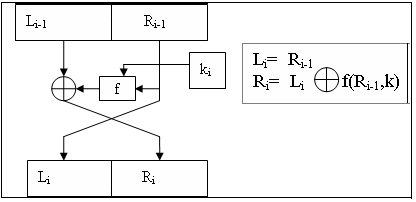
\includegraphics[scale=1.5]{pict/netF1.png}
\caption{Прямое преобразование сетью Фейстеля}
\end{figure}

\begin{figure}[H]
\centering
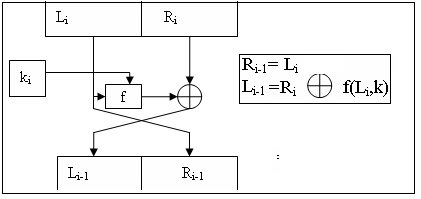
\includegraphics[scale=1.5]{pict/netF2.png}
\caption{Обратное преобразование сетью Фейстеля}
\end{figure}

\section{Схема шифрования алгоритма DES}
Схема шифрования алгоритма DES указана на Рисунке 1.3.
\begin{figure}[H]
\centering
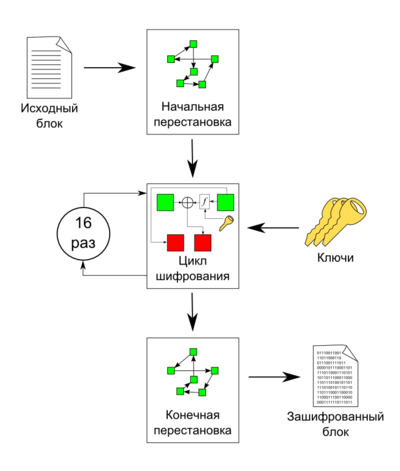
\includegraphics[scale=0.85]{pict/DES_algorithm_scheme.png}
\caption{Схема шифрования алгоритма DES}
\end{figure}

Исходный текст — блок 64 бит.

Процесс шифрования состоит из начальной перестановки, 16 циклов шифрования и конечной перестановки.

\subsection{Начальная перестановка}
Исходный текст \textbf{T} (блок 64 бит) преобразуется c помощью начальной перестановки \textbf{IP} которая определяется таблицей 1:
\begin{table}[H]
    \caption{Начальная перестанвока IP}
	\begin{tabular}{|c|c|c|c|c|c|c|c|c|c|c|c|c|c|c|c|}
    \hline
    58 & 50 & 42 & 34 & 26 & 18 & 10 & 2 & 60 & 52 & 44 & 36 & 28 & 20 & 12 & 4\\
    \hline
    62 &	54 &	46 &	38 &	30 &	22 &	14 &	6 &	64 &	56 &	48 &	40 &	32 &	24 &	16 &	8\\
    \hline
    57 &	49 &	41 &	33 &	25 &	17 &	9 &	1 &	59 &	51 &	43 &	35 &	27 &	19 &	11 &	3\\
    \hline
    61 &	53 &	45 &	37 &	29 &	21 &	13 &	5 &	63 &	55 &	47 &	39 &	31 &	23 &	15 &	7\\
    \hline
	\end{tabular}
\end{table}
По таблице первые 3 бита результирующего блока \textbf{IP(T)} после начальной перестановки \textbf{IP} являются битами 58, 50, 42 входного блока \textbf{T}, а его 3 последние бита являются битами 23, 15, 7 входного блока.

\subsection{Циклы шифрования}

Полученный после начальной перестановки 64-битовый блок IP(T) участвует в 16 циклах преобразования Фейстеля.

— 16 циклов преобразования Фейстеля:

Разбить IP(T) на две части $L_0,R_0$, где $L_0, R_0$ — соответственно 32 старших битов и 32 младших битов блока $T_0$ IP(T)= $L_0R_0$

Пусть $T_{i-1} = L_{i-1}R_{i-1}$ результат (i-1) итерации, тогда результат i-ой итерации $T_{i}=L_{i}R_{i}$ определяется:
\[L_{i}=R_{i-1}\]
\[R_{i}=L_{i-1}\oplus f(R_{i-1},k_{i})\]
Левая половина $L_{i}$ равна правой половине предыдущего вектора $L_{i-1}R_{i-1}$. А правая половина $R_{i}$ — это битовое сложение $L_{i-1}$ и $f(R_{i-1},k_{i})$ по модулю 2.

В 16-циклах преобразования Фейстеля функция f играет роль шифрования. Рассмотрим подробно функцию f.

\subsection{Основная функция шифрования (функция Фейстеля)}

Аргументами функции $f$ являются 32-битовый вектор $R_{i-1}$ и 48-битовый ключ $k_{i}$, который является результатом преобразования 56-битового исходного ключа шифра $k$. Для вычисления функции $f$ последовательно используются:
\begin{enumerate}
    \item функция расширения $E$,
    \item сложение по модулю 2 с ключом $k_i$
    \item преобразование $S$, состоящее из 8 преобразований $S$-блоков $S_{1}, S_{2}, S_{3 }\ldots S_8$,
    \item перестановка $P$.
\end{enumerate}

Функция $E$ расширяет 32-битовый вектор $R_{i-1}$ до 48-битового вектора $E(R_{i-1})$ путём дублирования некоторых битов из $R_{i-1}$; порядок битов вектора $E(R_{i-1})$ указан в таблице 2.
\begin{table}[H]
    \caption{Функция расширения E}
	\begin{tabular}{|c|c|c|c|c|c|}
    \hline
    32	& 1	& 2	& 3	& 4	& 5\\
    \hline
    4	& 5	& 6	& 7	& 8	& 9\\
    \hline
    8	& 9	& 10	& 11	& 12	& 13\\
    \hline
    12	& 13	& 14	& 15	& 16	& 17\\
    \hline
    16	& 17	& 18	& 19	& 20	& 21\\
    \hline
    20	& 21 &	22	& 23	& 24	& 25\\
    \hline
    24	& 25	& 26	& 27	& 28	& 29\\
    \hline
    28	& 29	& 30	& 31	& 32	& 1\\
    \hline
	\end{tabular}
\end{table}

Первые три бита вектора $E(R_{i-1})$ являются битами 32, 1, 2 вектора $R_{i-1}$. По таблице 2 видно, что биты 1, 4, 5, 8, 9, 12, 13, 16, 17, 20, 21, 24, 25, 28, 29, 32 дублируются. Последние 3 бита вектора $E(R_{i-1})$ — это биты 31, 32, 1 вектора $R_{i-1}$. Полученный после перестановки блок $E(R_{i-1})$ складывается по модулю 2 с ключами $k_i$ и затем представляется в виде восьми последовательных блоков $B_{1},B_{2},...B_{8}$.

\[E(R_{i-1})\oplus k_{i}=B_{1}B_{2}...B_{8}\]
Каждый $B_j$ является 6-битовым блоком. Далее каждый из блоков $B_j$ трансформируется в 4-битовый блок $B'_j$ с помощью преобразований $S_j$. Преобразования $S_j$ определяются на рисунке 1.4.

\begin{figure}[H]
\centering
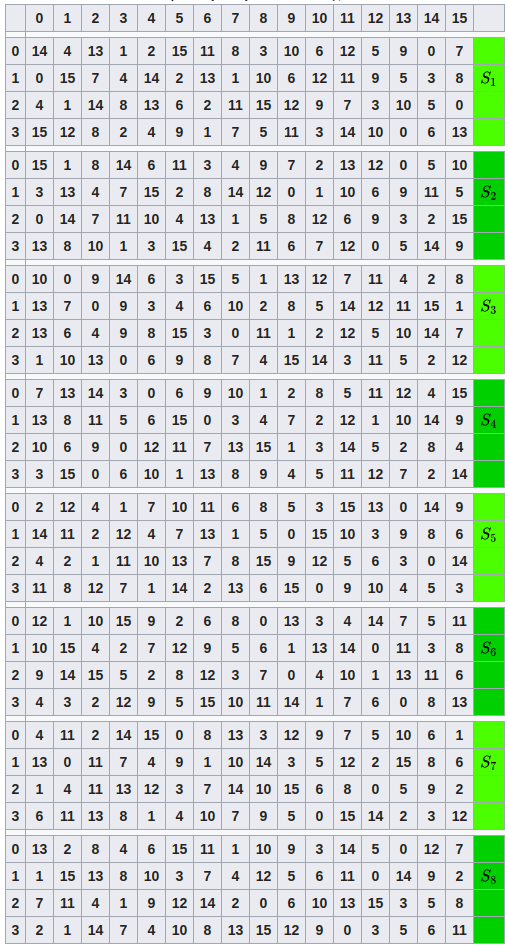
\includegraphics[scale=0.7]{pict/table.png}
\caption{Таблица 3. Преобразования $S_{i}, i=1…8$}
\end{figure}

Предположим, что $B_3 = 101111$, и мы хотим найти $B'_3$. Первый и последний разряды $B_{3}$ являются двоичной записью числа а, 0<=a<=3, средние 4 разряда представляют число b, 0<=b<=15. Строки таблицы S3 нумеруются от 0 до 3, столбцы таблицы S3 нумеруются от 0 до 15. Пара чисел (а, b) определяет число, находящееся в пересечении строки а и столбца b. Двоичное представление этого числа дает $B'_3$ . В нашем случае $a=11_{2}=3$, $b=0111_{2}=7$, а число, определяемое парой (3,7), равно 7. Его двоичное представление $B'_{3}$. Значение функции $f(R_{i-1},k_{i})$ (32 бит) получается перестановкой Р, применяемой к 32-битовому блоку $B'_{1}B'_{2}...B'_{8}$. Перестановка Р задана таблицей 3.

\begin{table}[H]
    \caption{Перестановка P}
	\begin{tabular}{|c|c|c|c|c|c|c|c|}
    \hline
    16	& 7	& 20	& 21	& 29	& 12	& 28	& 17\\
    \hline
    1	& 15	& 23	& 26	& 5	& 18	& 31	& 10\\
    \hline
    2	& 8	& 24	& 14	& 32	& 27	& 3	& 9\\
    \hline
    19	& 13	& 30	& 6	& 22	& 11	& 4	& 25\\
    \hline
	\end{tabular}
\end{table}

\[f(R_{i-1},k_i) = P(B'_1B'_2...B'_8)\]
Согласно таблице 4, первые четыре бита результирующего вектора после действия функции f — это биты 16, 7, 20, 21 вектора $B'_{1}B'_{2}...B'_{8}$

\subsection{Генерирование ключей $k_i$}

Ключи $k_i$ получаются из начального ключа $k$ (56 бит = 7 байтов или 7 символов в ASCII) следующим образом. Добавляются биты в позиции 8, 16, 24, 32, 40, 48, 56, 64 ключа $k$ таким образом, чтобы каждый байт содержал нечетное число единиц. Это используется для обнаружения ошибок при обмене и хранении ключей. Затем делают перестановку для расширенного ключа (кроме добавляемых битов 8, 16, 24, 32, 40, 48, 56, 64). Такая перестановка определена в таблице 4.
\begin{table}[H]
    \caption{Перестановка P}
	\begin{tabular}{|c|c|c|c|c|c|c|c|c|c|c|c|c|c|c|}
    \hline
    57	& 49	& 41	& 33	& 25	& 17	& 9	& 1	& 58	& 50	& 42	& 34	& 26	& 18 &	$C_{0}$\\
    \hline
    10	& 2	& 59	& 51	& 43	& 35	& 27	& 19	& 11	& 3	& 60	& 52	& 44	& 36 &\\
    \hline
    63	& 55	& 47	& 39	& 31	& 23	& 15	& 7	& 62 &	54	& 46	& 38	& 30	& 22 & $D_0$\\
    \hline
    14	& 6	& 61	& 53	& 45	& 37	& 29	& 21	& 13	& 5	& 28	& 20	& 12	& 4&\\
    \hline
    \end{tabular}
\end{table}

Эта перестановка определяется двумя блоками $C_{0}$ и $D_0$ по 28 бит каждый. Первые 3 бита $C_{0}$ есть биты 57, 49, 41 расширенного ключа. А первые три бита $D_0$ есть биты 63, 55, 47 расширенного ключа. $C_i, D_i i=1,2,3… $получаются из $C_{i-1}, D_{i-1}$ одним или двумя левыми циклическими сдвигами согласно таблице 5.
\begin{table}[H]
    \caption{}
	\begin{tabular}{|c|c|c|c|c|c|c|c|c|c|c|c|c|c|c|c|c|}
    \hline
    i	& 1	& 2	& 3	& 4	& 5	& 6	& 7	& 8	& 9	& 10	& 11	& 12	& 13	& 14	& 15	& 16\\
    \hline
    Число сдвига	& 1	& 1	& 2	& 2	& 2	& 2	& 2	& 2	& 1	& 2	& 2	& 2	& 2	& 2	& 2 &	1\\
    \hline
    \end{tabular}
\end{table}

Ключ $k_i$, i=1,…16 состоит из 48 бит, выбранных из битов вектора $C_{i}D_{i}$ (56 бит) согласно таблице 7. Первый и второй биты $k_i$ есть биты 14, 17 вектора $C_{i}D_{i}$

\begin{table}[H]
    \caption{}
	\begin{tabular}{|c|c|c|c|c|c|c|c|c|c|c|c|c|c|c|c|}
	\hline
	14	& 17	& 11	& 24	& 1	& 5	& 3	& 28	& 15	& 6	& 21	& 10	& 23	& 19	& 12	& 4\\
	\hline
	26	& 8	& 16	& 7	& 27	& 20	& 13 &	2	& 41	& 52	& 31	& 37	& 47	& 55	& 30	& 40\\
	\hline
	51	& 45	& 33	& 48	& 44	& 49	& 39	& 56	& 34	& 53	& 46	& 42	& 50	& 36	& 29	& 32\\
	\hline
	\end{tabular}
\end{table}

\subsection{Конечная перестановка}
Конечная перестановка $IP^{-1}$ действует на $T_{16}$ и является обратной к первоначальной перестановке. Конечная перестановка определяется таблицей 1.7.
\begin{table}[H]
	\caption{}
	\begin{tabular}{|c|c|c|c|c|c|c|c|c|c|c|c|c|c|c|c|}
	\hline
	40  & 8  & 48 & 16 & 56 & 24 & 64 & 32 & 39 & 7 &  47 & 15 & 55 & 23 & 63 & 31\\
	\hline
	38 & 6  & 46 & 14 & 54 & 22 & 62 & 30 & 37 & 5  & 45 & 13 & 53 & 21 & 61 & 29\\
	\hline
	36 & 4  & 44 & 12 & 52 & 20 & 60 & 28 & 35 & 3  & 43 & 11 & 51 & 19 & 59 & 27\\
	\hline
	34 & 2  & 42 & 10 & 50 & 18 & 58 & 26 & 33 & 1  & 41 & 9  & 49 & 17 & 57 & 25\\
	\hline
	\end{tabular}
\end{table}

\DeclareGraphicsExtensions{.pdf,.png,.jpg}

\chapter{Конструкторский раздел}
\label{cha:design}

В данном разделе будет произведена конкретизация задач и проанализированы алгоритм.

\section{IDEF0 Модель}

На рисунке 2.1 приведена функциональная модель шифрования в нотации IDEF0.
\begin{figure}[H]
\centering
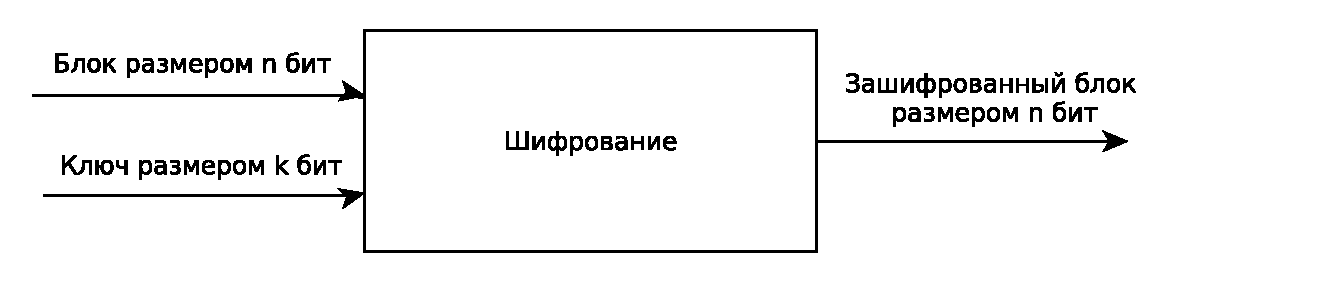
\includegraphics[scale=0.75]{./pict/ideftr.pdf}
\caption{Функциональная модель шифрования}
\end{figure}
\newpage

\section{Разработка алгоритмов}
Подробная схема шифрования алгоритма DES представленна на рисунке 2.2.

\begin{figure}[H]
\centering
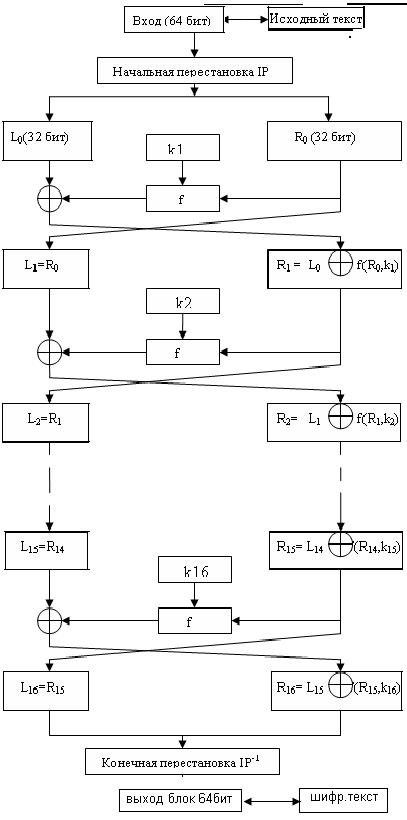
\includegraphics[scale=1.2]{./pict/Code.png}
\caption{Алгоритм DES}
\end{figure}

\section{Вывод}
В данном разделе была рассмотрена схема алгоритма.

\chapter{Технологический раздел}
\label{cha:impl}

В данном разделе приводятся описания требований к программному обеспечению, средства реализации, листинги кода и описания тестирования.
\section{Требования к программному обеспечению}
Требования к вводу:
\begin{itemize}
    \item на вход подается массив;
\end{itemize}
Требования к выводу:
\begin{itemize}
    \item на выход подаются массивы, отсортированные разными алгоритмами;
\end{itemize}
\section{Средства реализации}
В качестве языка программирования мною был выбран python, так как данный язык программирования позволяет максимально лаконично и демонстративно реализовать необходимые алгоритмы.
\section{Листинги кода}

В листингах 3.1 - 3.3 приведена реализация описанных алгоритмов.
\begin{lstlisting}[caption=Поразрядная сортировка]
	n = pow(digit, n)
    	i = 1
    	while (i < n):
		sort = [[] for k in range(digit)]

		for x in array:
			sort[get_digit(x, i)].append(x)

		count = len(array)
		array = [0] * count
		u = 0
		w = 0
		for k in range(digit):
			for j in range(len(sort[k])):
				if (sort[k][j] < 0):
					array[w] = sort[k][j]
					w += 1
				else:
					array[u + neg] = sort[k][j]
					u += 1
		i *= 10
\end{lstlisting}

\begin{lstlisting}[caption=Сортировка вставками]
	for i in range(1, len(array)):
		j = i - 1
		key = array[i]
		while array[j] > key and j >= 0:
			array[j + 1] = array[j]
			j -= 1
		array[j + 1] = key
\end{lstlisting}

\noindent\begin{minipage}{\textwidth}
\begin{lstlisting}[caption=Быстрая сортировка]
def partition(nums, low, high):
    middle = nums[(low + high) // 2]
    i = low - 1
    j = high + 1
    while True:
        i += 1
        while nums[i] < middle:
            i += 1
        j -= 1
        while nums[j] > middle:
            j -= 1
        if i >= j:
            return j
        nums[i], nums[j] = nums[j], nums[i]

def quicking_sort(items, low, high):
    if low < high:
        split_index = partition(items, low, high)
        quicking_sort(items, low, split_index)
        quicking_sort(items, split_index + 1, high)

def quick_sort(nums):
    quicking_sort(nums, 0, len(nums) - 1)
\end{lstlisting}
\end{minipage}

\section{Описание тестирования}
Для тестирования программы были подготовлены данные, представленные в таблице 1.
	\begin{center}
		\begin{tabular}{  | c | c | }
			\hline
			\textbf{Маcсив}& \textbf{Ожидаемый результат} \\ \hline
			$\begin{bmatrix} 
   			1&2&3 \\
			\end{bmatrix}$ & 
			$\begin{bmatrix} 
   			1&2&3 \\
			\end{bmatrix}$ \\
			\hline
			
			$\begin{bmatrix} 
   			3&2&1 \\
			\end{bmatrix}$ & 
			$\begin{bmatrix} 
   			1&2&3 \\
			\end{bmatrix}$ \\
			\hline
			
			$\begin{bmatrix} 
   			1&2&-3 \\
			\end{bmatrix}$ & 
			$\begin{bmatrix} 
   			-3&1&2 \\
			\end{bmatrix}$ \\
			\hline
			
			$\begin{bmatrix} 
   			1&0&-3 \\
			\end{bmatrix}$ & 
			$\begin{bmatrix} 
   			-3&0&1 \\
			\end{bmatrix}$ \\
			\hline
			
			$\begin{bmatrix} 
   			0 \\
			\end{bmatrix}$ & 
			$\begin{bmatrix} 
   			0 \\
			\end{bmatrix}$ \\
			\hline
		\end{tabular}
		
		\hfill
		
		Таблица 1.
		Подготовленные тестовые данные.  
	\end{center}
	
Все тесты были успешно пройдены.
\section{Вывод}

Были сформулированы требования к ПО, выбраны средства реализации и подготовлены тестовые данные.
%%%% mode: latex
%%%% TeX-master: "rpz"
%%%% End:

\chapter{Исследовательский раздел}
\label{cha:research}

В данном разделе привидены и проанализированы примеры работы реализованной программы.


Исследования проводились на компьютере следующей конфигурации:
- процессор Intel Core i7-7700 2.80 GHz, 4 логических ядра;
– ОЗУ 8Гб;
– ОС Ubuntu 18.04.
\section{Примеры работы}

На рисунках 4.1, 4.2, 4.3 показана работа программы с различными входными данными.


\begin{figure}[H]
\centering
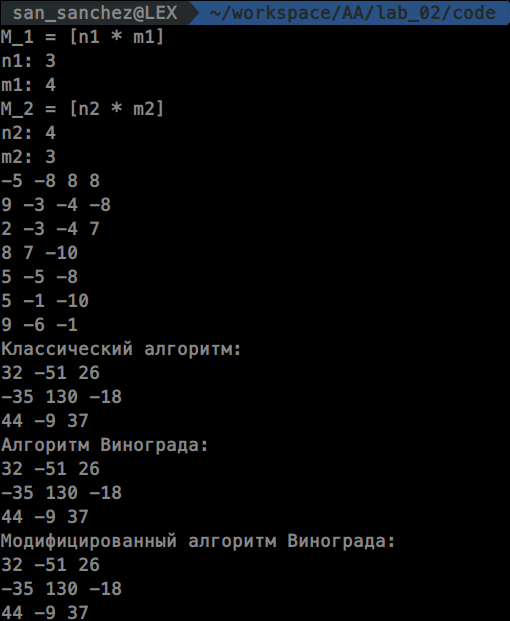
\includegraphics[scale=0.75]{./pictures/wrk2.png}
\caption{Тест на неверный ввод}
\end{figure}
\begin{figure}[H]
\centering
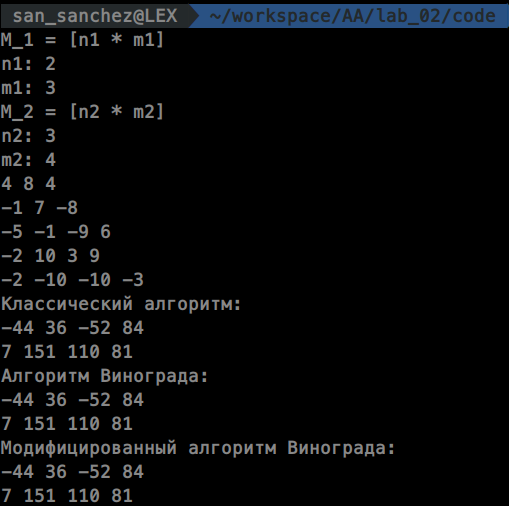
\includegraphics[scale=0.75]{./pictures/wrk3.png}
\caption{Тест на верных входных данных}
\end{figure}
\begin{figure}[H]
\centering
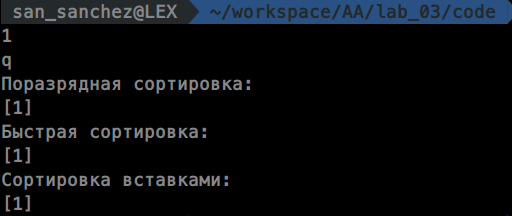
\includegraphics[scale=0.75]{./pictures/wrk5.png}
\caption{Тест при вводе всего одного элемента}
\end{figure}

\newpage
\section{Эксперименты по замеру времени}
На графиках 6-7 представлено сравнение алгоритмов умножения матриц. 
	\begin{center}
        		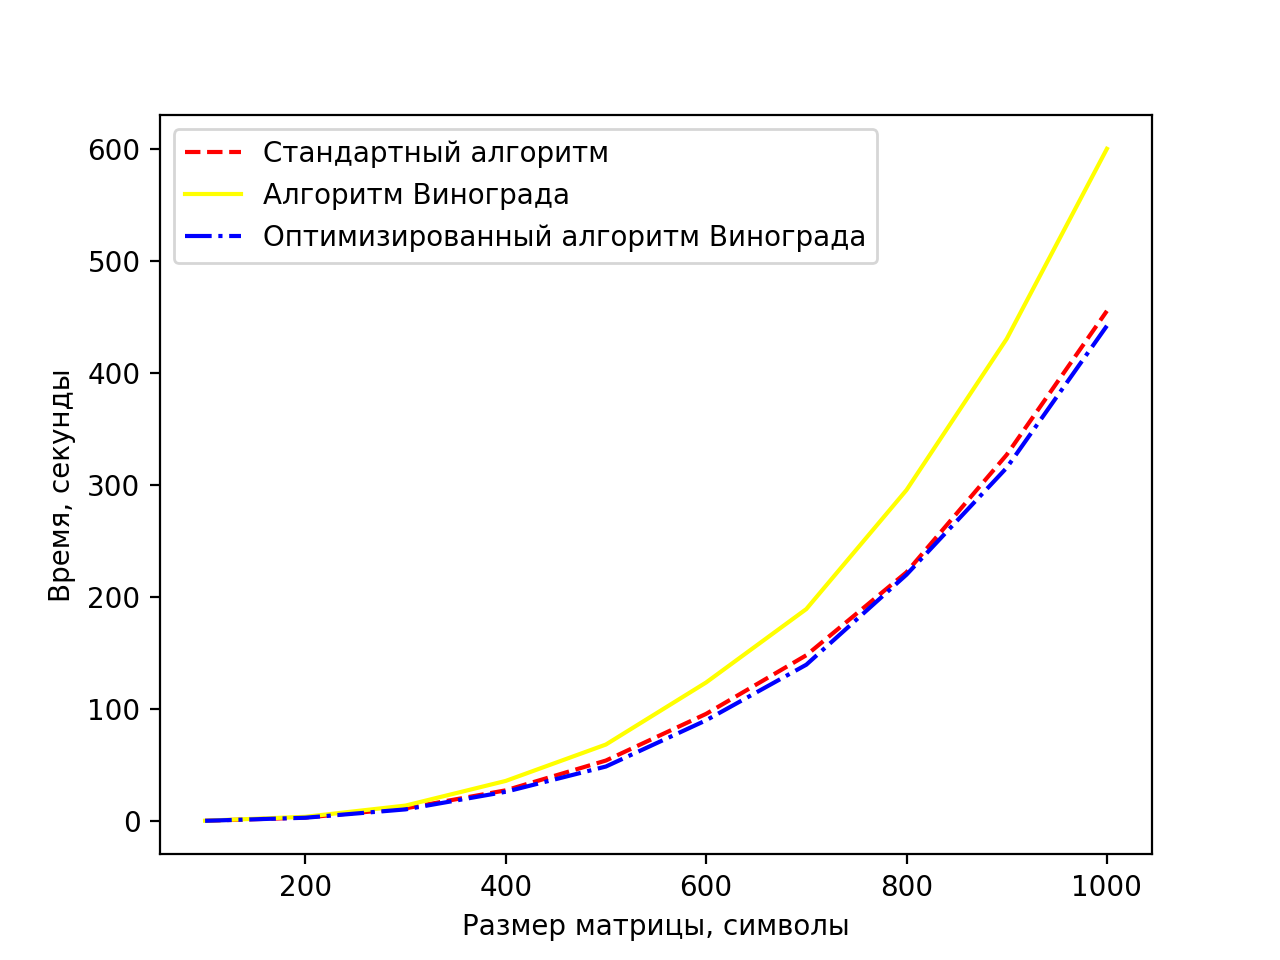
\includegraphics[scale = 1]{./pictures/graph1} \\ Рис. 4.4 - Сравнение реализации алгоритмов сортировок на произвольных данных.
	\end{center}
	
	\begin{center}
        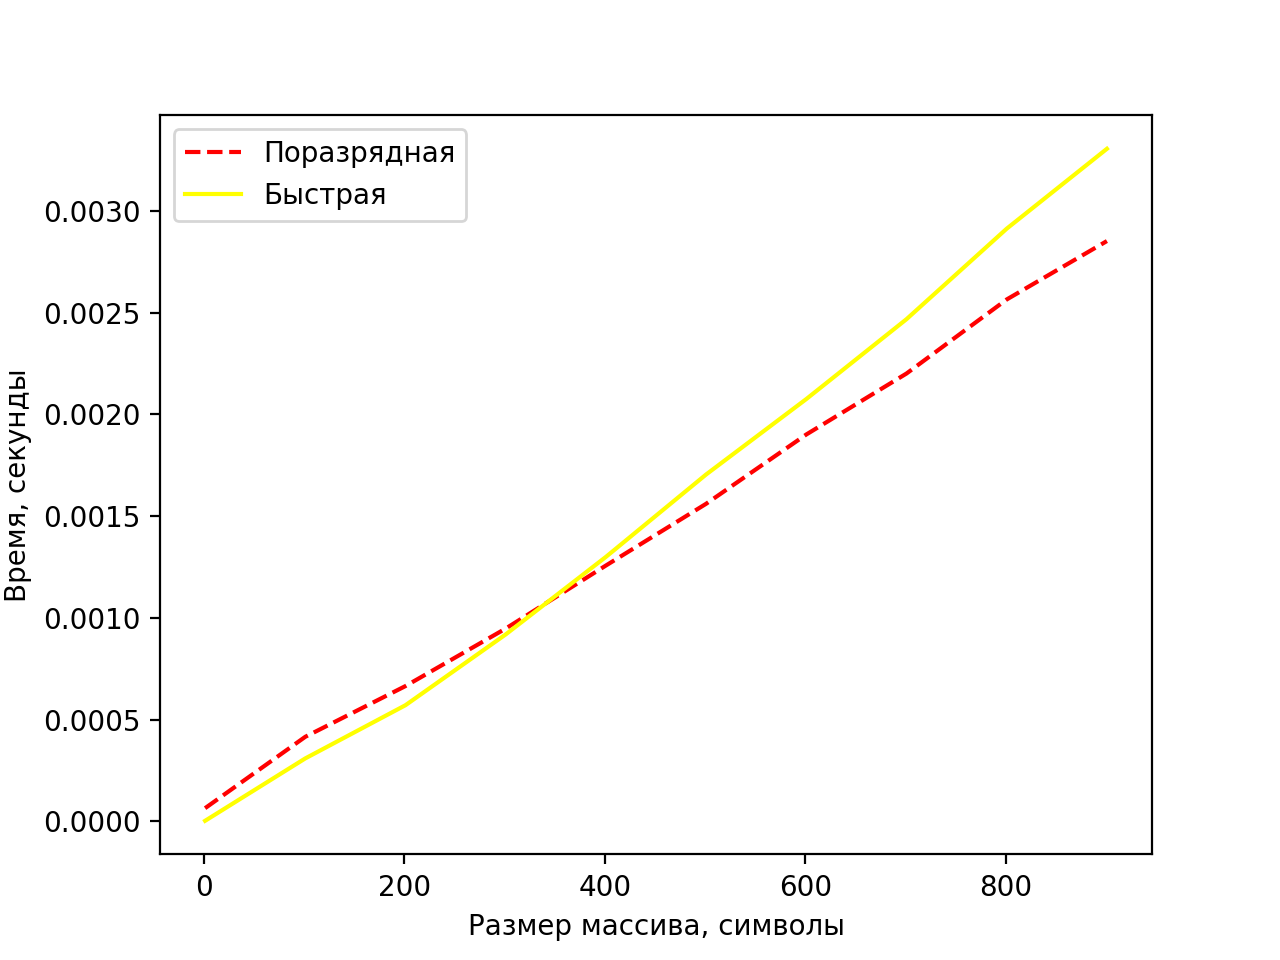
\includegraphics[scale = 1]{./pictures/graph2} \\ Рис. 4.5 - Сравнение реализации алгоритмов сортировок быстрой и поразрядной на произвольных данных(при
        средней разрядности числа до 4 значащих цифр).
	\end{center}
	\begin{center}
        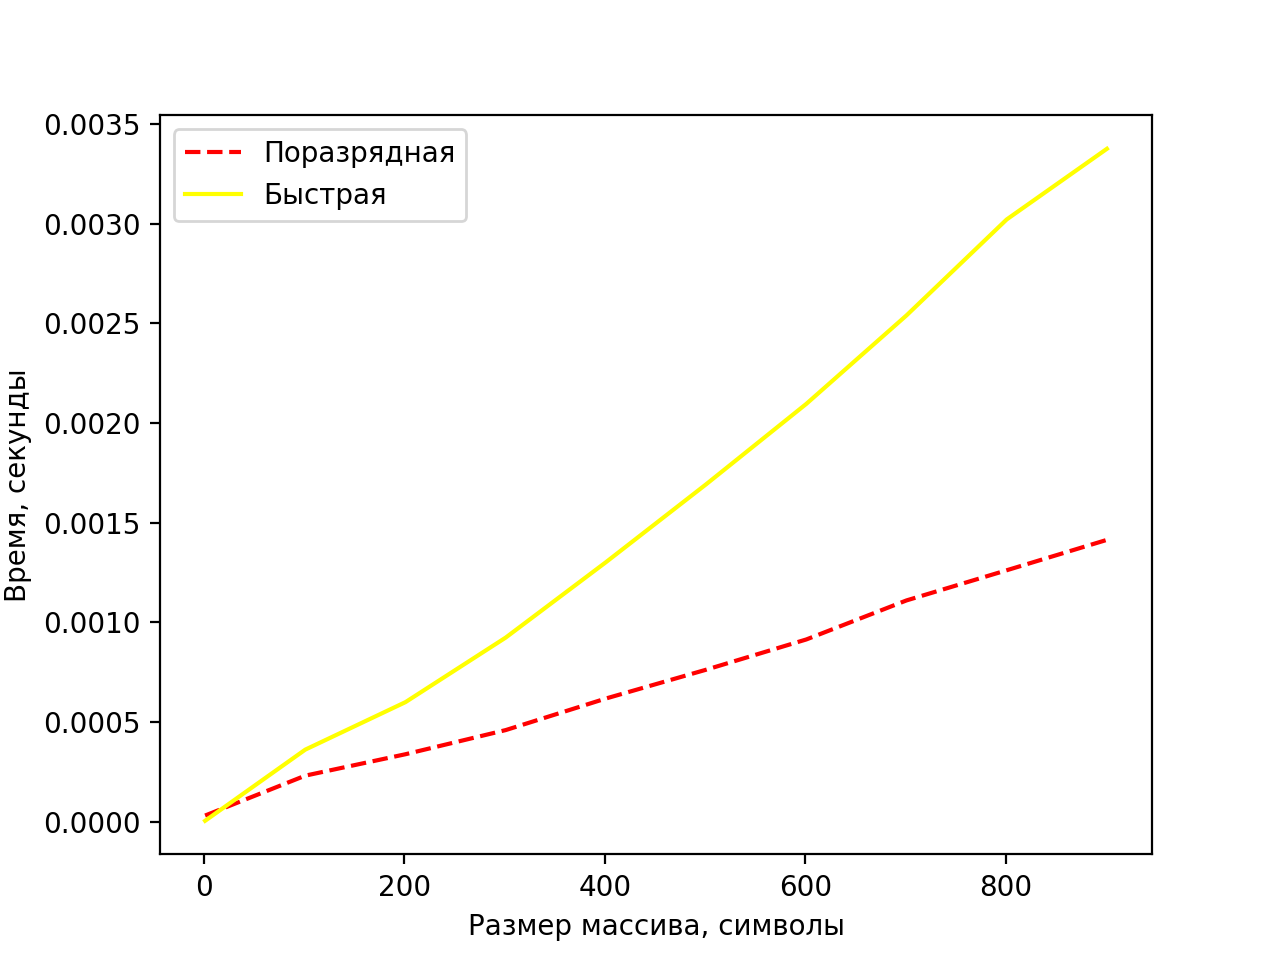
\includegraphics[scale = 1]{./pictures/graph3} \\ Рис. 4.6 - Сравнение реализации алгоритмов сортировок быстрой и поразрядной на произвольных данных (при
        маленькой разрядности числа 1 значащая цифра).
	\end{center}
	\begin{center}
        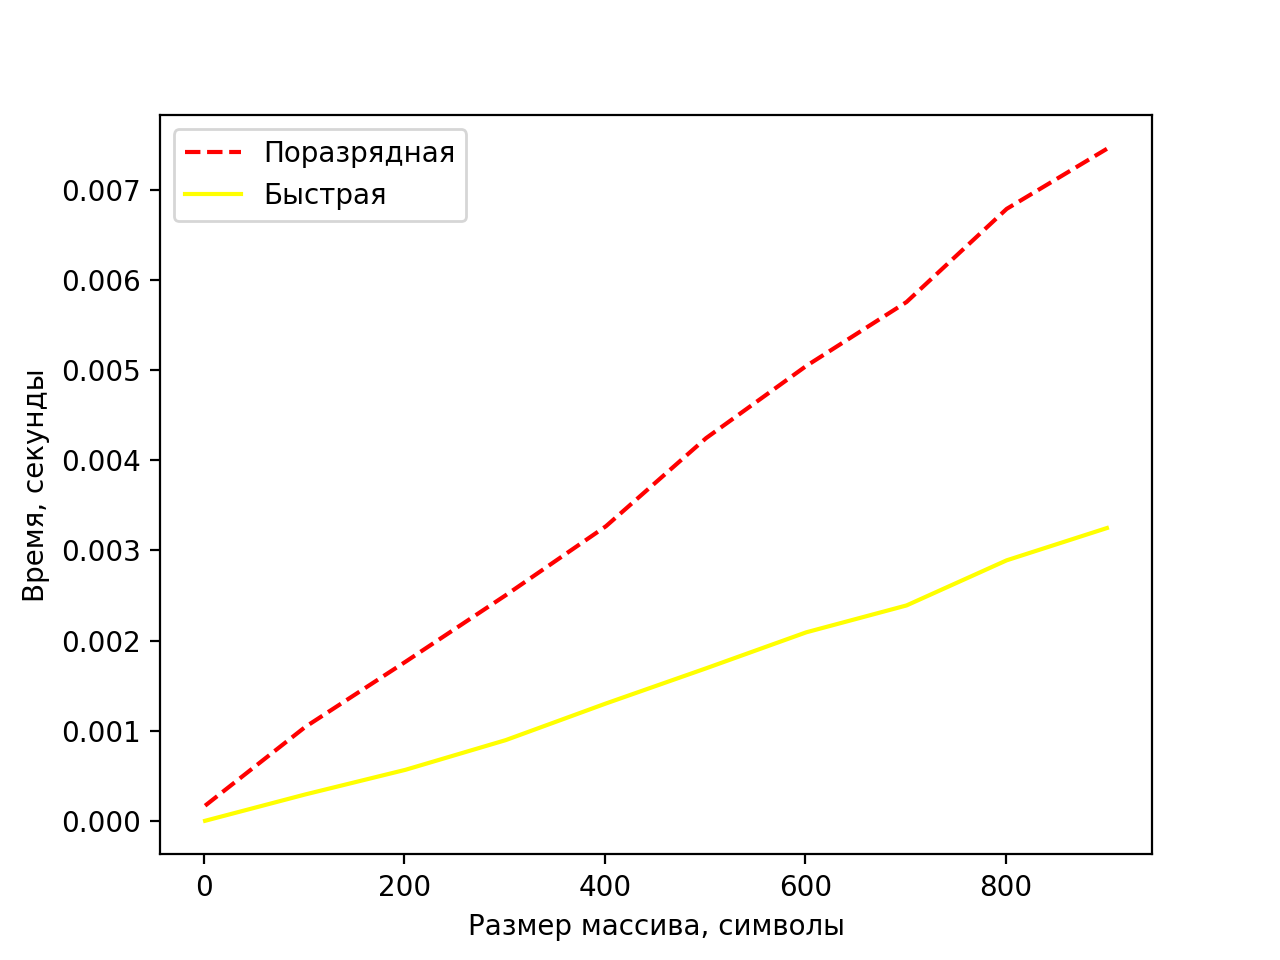
\includegraphics[scale = 1]{./pictures/graph4} \\ Рис. 4.7 - Сравнение реализации алгоритмов сортировок быстрой и поразрядной на произвольных данных (при
        большой разрядности числа до 10 значащих цифр).
	\end{center}
	\begin{center}
        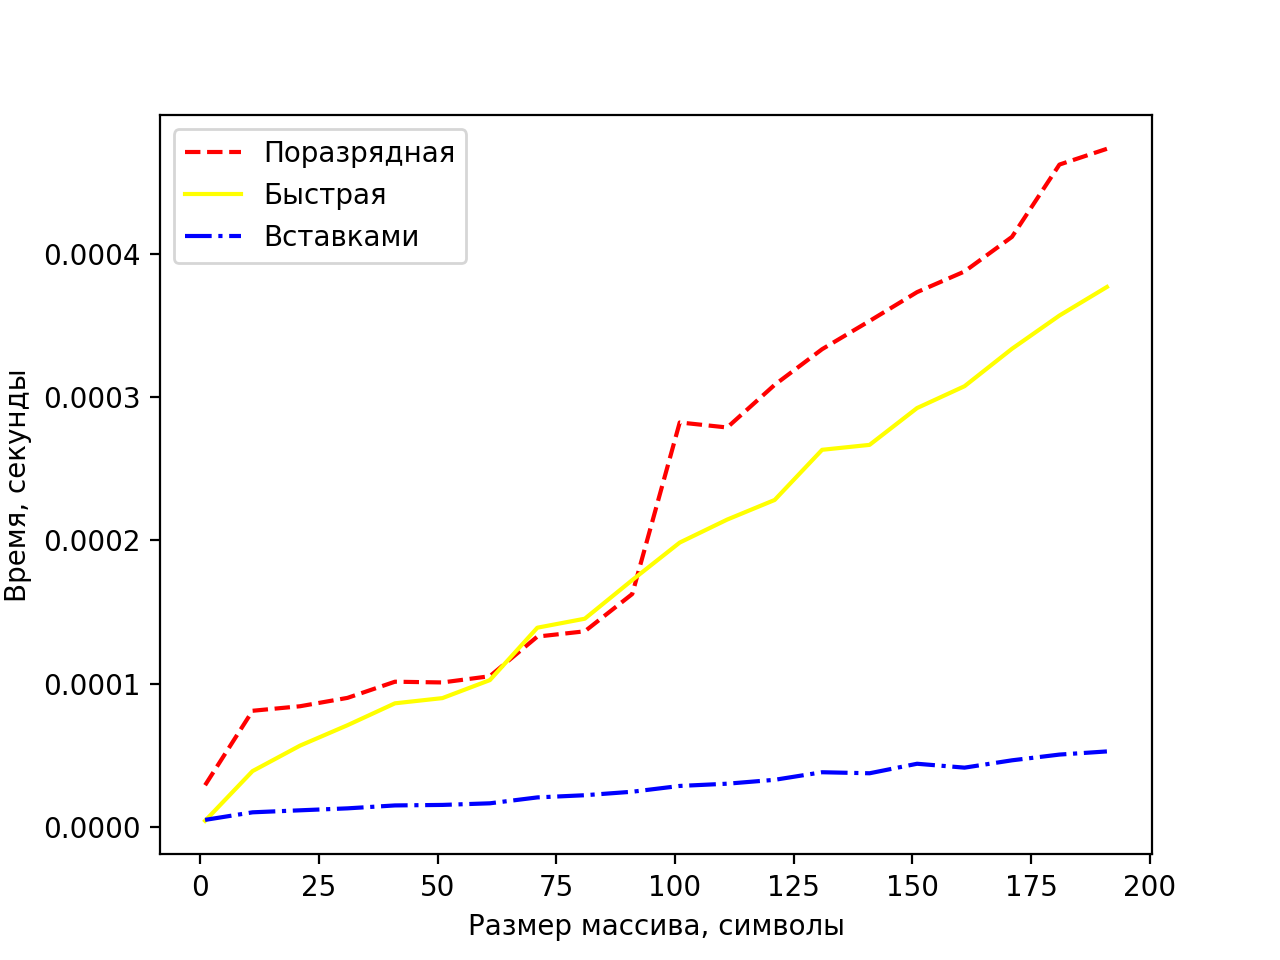
\includegraphics[scale = 1]{./pictures/graph5} \\ Рис. 4.8 - Сравнение реализации алгоритмов сортировок на упорядоченных данных.
	\end{center}
	\begin{center}
        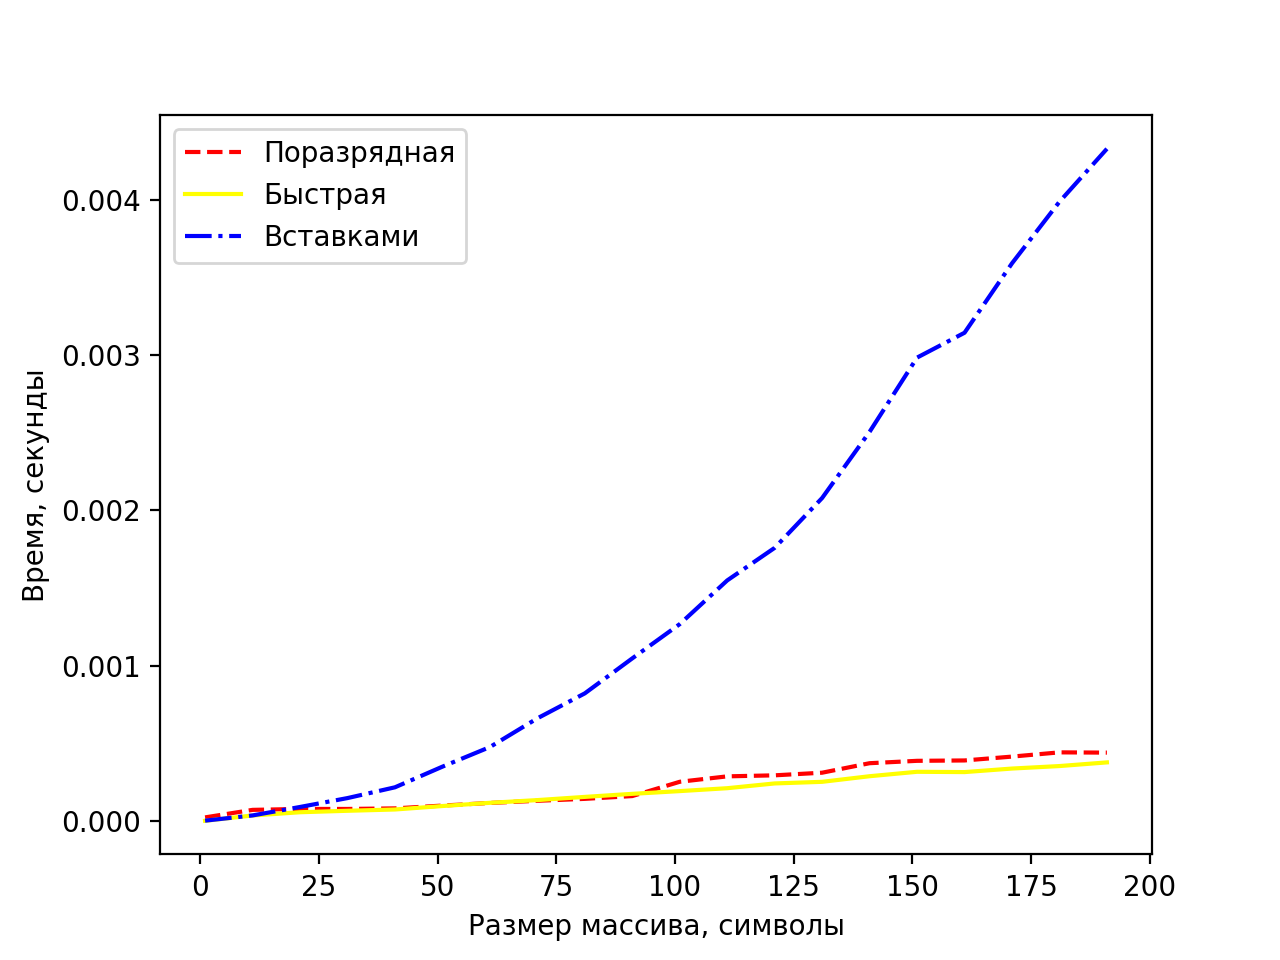
\includegraphics[scale = 1]{./pictures/graph6} \\ Рис. 4.9 - Сравнение реализации алгоритмов сортировок на обратно упорядоченных данных.
	\end{center}
	\begin{center}
        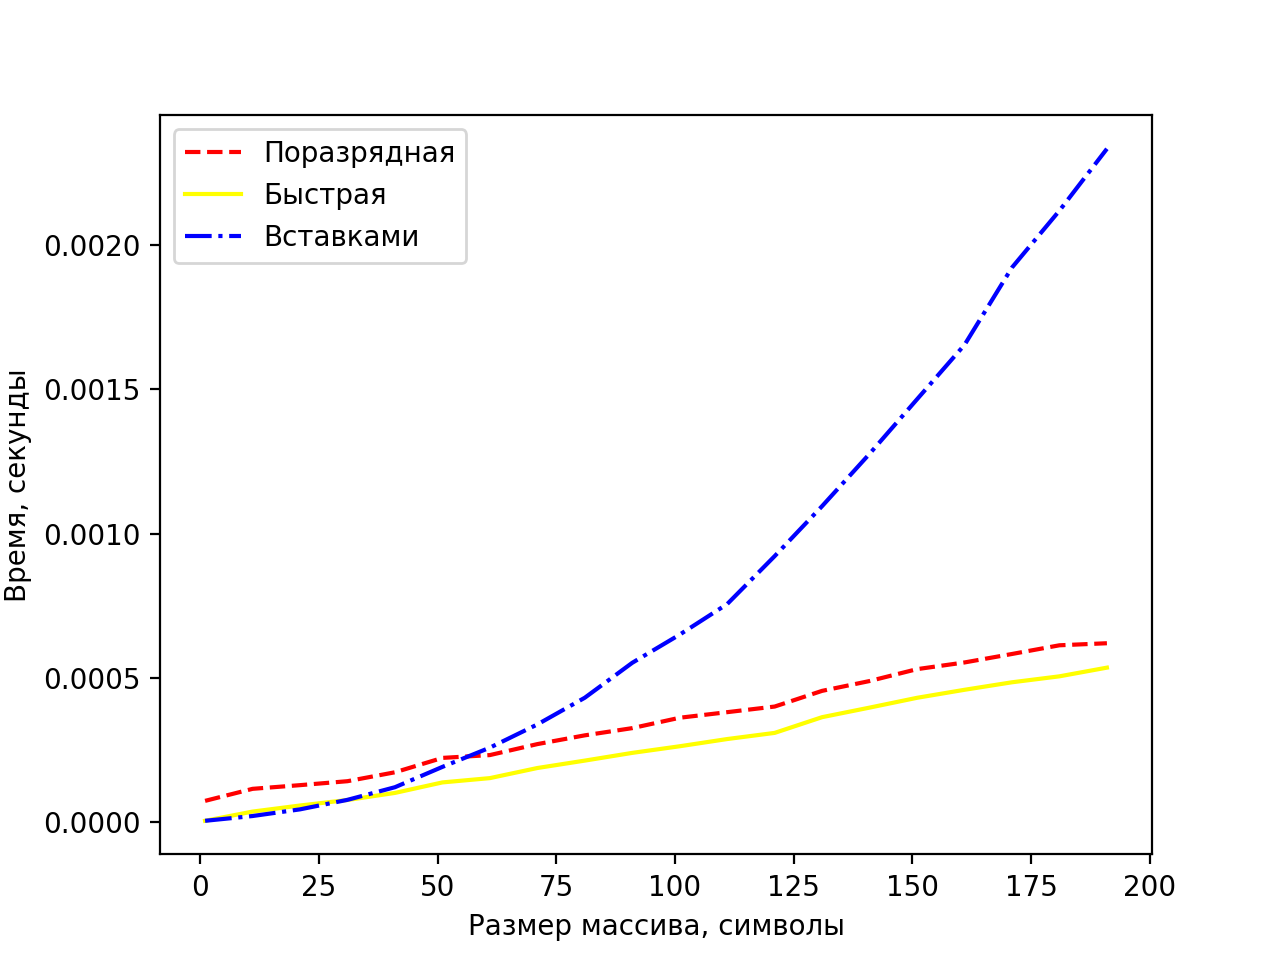
\includegraphics[scale = 1]{./pictures/graph7} \\ Рис. 4.10 - Сравнение реализации алгоритмов сортировок на произвольных данных при небольших размерах
        массивов.
	\end{center}
\section{Выводы}
Как видно из графиков и из проведенного анализа трудоемкости, поразрядная сортировка имеет
линейную зависимость от длины массива и разрядности элементов; быстрая - квадаратичную в худшем
случае и 𝑛 · 𝑙𝑜𝑔(𝑛) - в остальных; поразрядная - линейную в лучшем и квадратичную в среднем и худшем
случаях.
\pagebreak



\backmatter %% Здесь заканчивается нумерованная часть документа и начинаются ссылки и
            
\Conclusion % заключение к отчёту
В ходе даннои работы были изучены алгоритмы поразрядной и быстрой сортировок, сортировки
вставками; были получены практические навыки реализации указанных алгоритмов. Была проведена
оценка сложности теоретически с указанием лучшего и худшего случаев (если есть) и условий их наступления. Был проведен сравнительный анализ перечисленных алгоритмов сортировки по затрачиваемым
ресурсам времени и получено экспериментальное подтверждение различий во временн´oй эффективности
выбранных алгоритмов сортировки при помощи разработанного программного обеспечения на материале
замеров процессорного времени выполнения реализации на варьирующихся длинах массивов. В результате были получены следующие выводы:
\begin{enumerate}

	\item Сортировка вставками работает медленнее остальных исследуемых алгоритмов при во всех рассмотренных случаях на длинных массивах (≈ от 100 элементов). Но этот алгоритм эффективен на
небольших наборах данных, на наборах данных до десятков элементов может оказаться лучшим;
он также эффективен на наборах данных, которые уже частично отсортированы; это устойчивый
алгоритм сортировки (не меняет порядок элементов, которые уже отсортированы);
	\item Основным достоинством поразрядной сортировки является скорость, однако она требует использования дополнительной памяти и имеет узкую специализацию;
	\item	Алгоритм быстрой сортировки является одним из самых быстрых универсальных алгоритмов сортировки массивов. Однако в худшем случае глубина рекурсии при выполнении алгоритма достигнет n,
что будет означать n-кратное сохранение адреса возврата и локальных переменных процедуры разделения массивов. Для больших значений n худший случай может привести к исчерпанию памяти
(переполнению стека) во время работы программы.
\end{enumerate}
%% заключение

% % Список литературы при помощи BibTeX
% Юзать так:
%
% pdflatex rpz
% bibtex rpz
% pdflatex rpz

\bibliographystyle{ugost2008}
\bibliography{rpz}
\begin{enumerate}
\bibitem{} Сортировка таблицы [Электронный ресурс]. - Режим доступа: https://support.office.com/ru-ru/article/
\bibitem{} Кнут Д. Э., Козаченко Ю. В., Красиков И. В. Искусство программирования: Сортировка и поиск. Классический труд, Т. 3. М. : Вильямс, 2000. –– 824 c.
\bibitem{}  Sorting Benchmarks [Электронный ресурс]. - Режим доступа: http://sortbenchmark.org/ (дата обращения: 19.10.2019)
\bibitem{}  Алгоритмы сортировки [Электронный ресурс]. - Режим доступа: http://kit.znu.edu.ua/Meth/SORTALG.pdf (дата обращения: 19.10.2019)
\bibitem{} Алгоритм сортировки [Электронный ресурс]. - Режим доступа: https://www.wikiwand.com/ru/Алгоритмсортировки (дата обращения: 19.10.2019)
\bibitem{}  Алгоритмы сортировки в народных танцах [Электронный ресурс]. - Режим доступа: https://forany.xyz/a-370 (дата обращения: 19.10.2019)
\bibitem{}  Сортировка данных [Электронный ресурс]. - Режим доступа: http://www.hpcc.unn.ru/mskurs/RUS/DOC/ppr10.pdf (дата обращения: 19.10.2019)
\end{enumerate}
%%% Local Variables: 
%%% mode: latex
%%% TeX-master: "rpz"
%%% End: 

\bibliographystyle{ugost2008}
\bibliography{rpz}
\begin{enumerate}
    \item А. П. Алферов, А. Ю. Зубов, А. С. Кузьмин, А. В. Черемушкин . Основы криптографии.
    \item A. Menezes, Pvan Oorschot, S. Vanstone. Handbook of Applied Cryptography.
    \item Семенов Ю. А. Алгоритм DES.
\end{enumerate}

%
%
%\chapter{Еще картинки}
\label{cha:appendix2}
\blindtext

\begin{figure}
\centering
\caption{Еще одна картинка, ничем не лучше предыдущей. Но надо же как-то заполнить место.}
\end{figure}

%%% Local Variables: 
%%% mode: latex
%%% TeX-master: "rpz"
%%% End: 


\end{document}

%%% Local Variables:
%%% mode: latex
%%% TeX-master: t
%%% End:
